\Chapter{Gesztusok}

\Section{Felismerendő gesztusok}

A szoftver használata közben a prezentáló személy különféle gesztusok segítségével léphet kapcsolatba a virtuális elemekkel. Általában a felhasználó a karjai mozgatásával valósítja meg ezeket a mozdulatokat.

\begin{itemize}
\item \textbf{Sweep}: Egyenes vonalú mozgás. A mozgásnak van iránya és két képkocka között megfigyelhető a hossza is.
\item \textbf{Shift}: Bizonyos virtuális elemek közvetlenül is reagálnak a környezetükben történő mozgásra. Az ilyen elemek az irányukba történő mozgásra ellentétes irányú mozgással reagálnak. Vagyis a prezentáló személy például a kezei segítségével egyszerűen eltolhatja az adott virtuális elemet.
\item \textbf{Blink}: Az ujjak gyors ökölbe zárása és a tenyér széttárásának mozdulata.
\item \textbf{Drag}: Bizonyos virtuális elemeket a prezentáló személy képes megfogni, majd odébbhúzni és elengedni. A funkció eléréséhez a prezentálónak egy \textit{Blink} gesztust kell végrehajtania. Az elkapás pillanatában az adott objektum a \textit{Blink} pozíciójára (a prezentáló kézefére) tapad és követi annak helyzetét. A felhasználó így tetszőleges irányba mozgathatja az "elkapott" elemet. Egy újabb \textit{Blink} gesztussal pedig a kívánt helyére teheti azt.
\item \textbf{Rotation}: A videófolyamon történő örvénylő mozgás, ami akár több ponton is megfigyelhető.
\end{itemize}

\Section{Képek és vektor mezők}

Az elmozdulás becslésére az ún. Motion-Flow technikák tűntek a legalkalmasabbnak, azokból kiemelkedő eljárás a Bruce D. Lucas és Takeo Kanade által kidolgozott módszer, melynek implementálása az OpenCV-ben is megtalálható.

\cite{lucas1981iterative}
Flow Motion működésének a leírása a cikk alapján...
Részletezés képletekkel, ábrákkal...

Elmozdulás becslésének módja...

\Section{Rácspontok kezelése}

Ha az \textit{Optical-Flow} eljárást tetszőleges számú pontra elvégezhetjük. Ha létrehozhatunk egy rácsszerkezetet fix pontokkal, akkor a képtartományt egyenletesen lefedhetjük a pontok halmazával.
Ezen pontokat felhasználva minden iterációban az éppen aktuális és az egyel korábbi szürkeárnyalatos képkockákra elvégezhetjük az eljárást és így minden esetben kapunk egy új ponthalmazt, amely az eljárás eredménypontjait tartalmazza. Az eredeti és az új pontokból egy vektormezőt kapunk.

\begin{figure}[h]
\centering
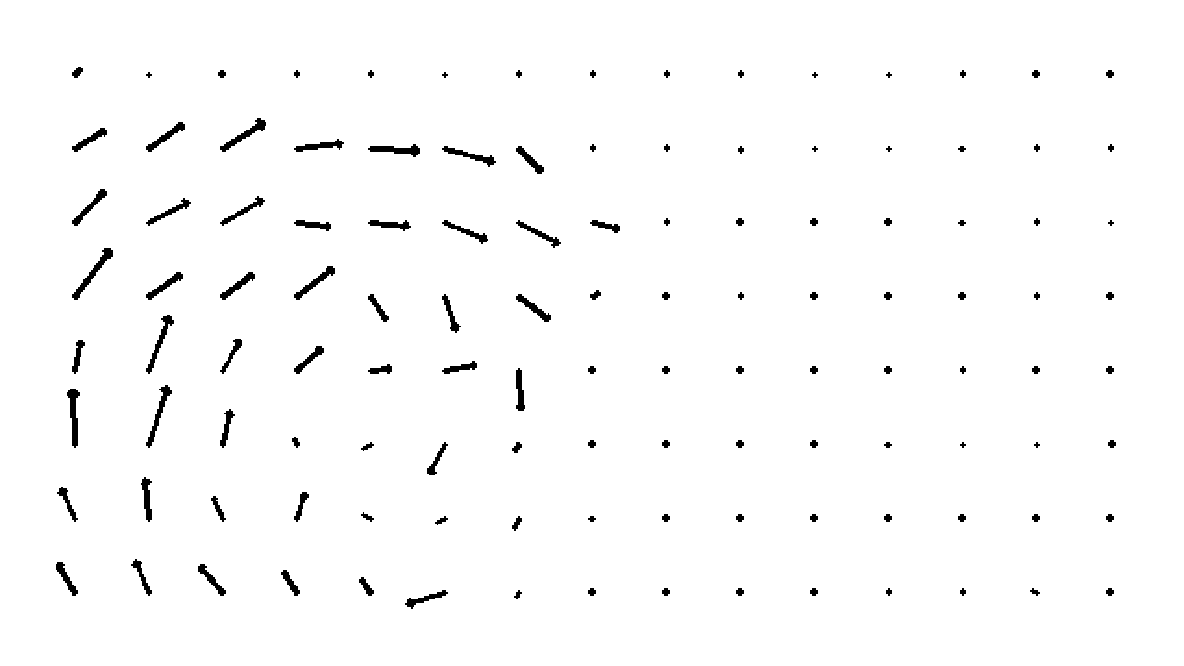
\includegraphics[width=11.2truecm, height=6.3truecm]{images/vectorField_screenshot.png}
\caption{Képernyőfotó a vektormezőről}
\label{fig:vectorfield}
\end{figure}

A mozgás detektálása rácspontok segítségével kevesebb számítást igényel, mintha minden pixel elmozdulását vizsgálnánk és az elmozdulás becslésére is elfogadható eredményeket kapunk.
A rács sűrűségét tetszőlegesen megadhatjuk. Minél sűrűbb a rács szerkezete, annál több pontot vizsgál a szoftver, ami nagyobb pontosságot is eredményez. Viszont a sűrűbb rács használata a futási időt is befolyásolja. Egy gyengébb hardver esetén nem ajánlott magas sűrűség értékkel futatnunk a programot, mivel tapasztalataim szerint jelentős lassulásra számíthatunk.

Hogyan számolja ki a kezdeti rácspontok helyzetét? 
\newpage
\Section{Hőtérkép}

A vektormező egyes pontjait vizsgálva szerkeszthetünk egy ún. \textit{Hőtérkép}-et, amelyben különböző intenzitásértékekkel jelöljök az egyes vektorok hosszait. A \textit{Hőtérkép} egy $n*m$-es mátrix, ahol $n$ a vektormező sorainak, $m$ pedig az oszlopainak a száma. A \textit{Hőtérkép} minden eleme egy BGR (blue, green, red) hármas értékkel van ellátva. Ezen értékek jelölik az egyes elemek színét.\\
Az értékek a következőképpen kerülnek kiszámításra:
\begin{align*}
  \textit{hőérték}_{nm} &= \textit{hossz}(\textit{vektor}_{nm})*\textit{nagyítás}\\
  \textit{hőtérkép}_{nm} &= (255-\textit{hőérték}_{nm},\ 0,\ \textit{hőérték}_{nm})
\end{align*}
0 pixel hosszúság esetén az adott indexű elem (255, 0, 0) értéket kap, vagyis kék színnel jelöljük. Ha egy adott vektor számított hőértéke eléri a 255-öt, a hozzá tartozó \textit{hőtérkép-érték} (0, 0, 255) intenzitásértéket kap, vagyis tiszta piros színnel fog megjelenni.
A \textit{nagyítás} mértéke jelenleg 10... \textbf{Ezt majd pontosítani kell, hogy honnan jön ez az érték!}

\begin{figure}[h]
\centering
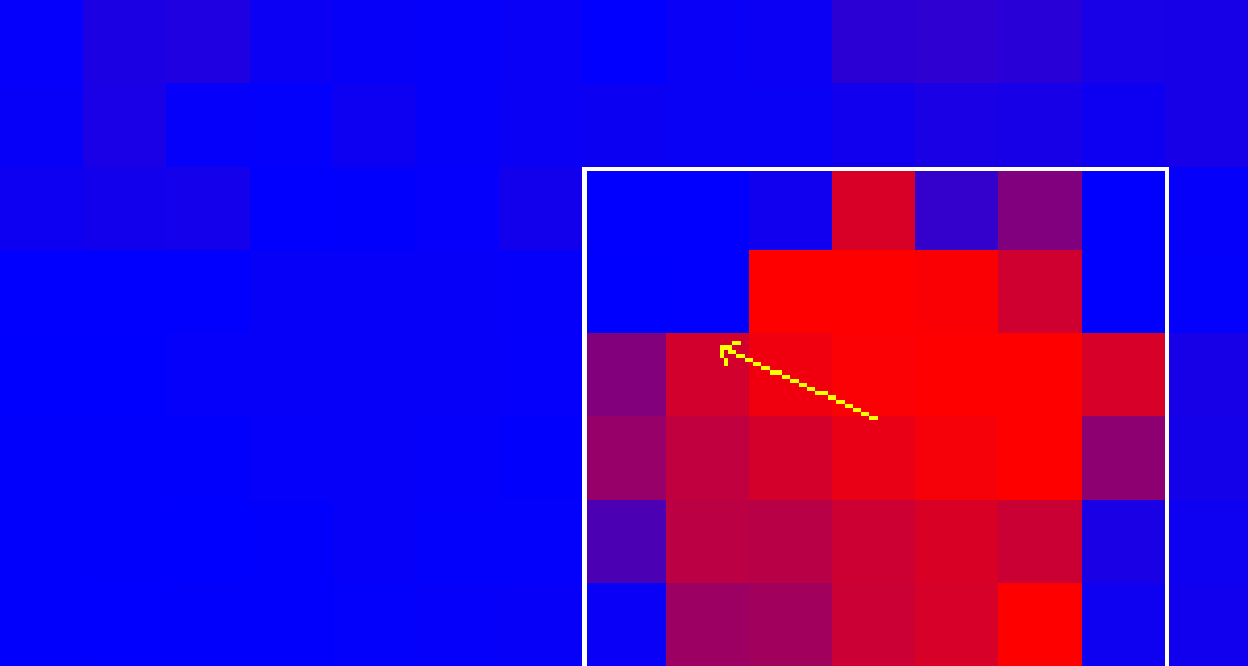
\includegraphics[width=11.2truecm, height=6.3truecm]{images/HeatMap_screenshot.png}
\caption{Képernyőfotó a hőtérképről}
\label{fig:heatmap}
\end{figure}

\Section{Kontrollpontok és vektorok számítása}

\SubSection{Sweep}

\SubSection{Shift}

\SubSection{Drag}

\SubSection{Blink}

\SubSection{Rotation}
